\documentclass[9pt, a4paper, ngerman]{arbeitsblatt}

\ladeModule{theme,qrcodes,boxen}

\ladeFach[quelltexte,uml]{informatik}
\ladeFach[geometrie,vektoren]{mathematik}

\aboptionen{
	name		= {J. Neugebauer},
	kuerzel 	= {Ngb},
	titel 		= {Physiksimulation in Processing},
	reihe 		= {Objektorientierte Programmierung},
	fach 		= {Informatik},
	kurs 		= {EF},
	nummer 		= {IV.0},
	lizenz 		= {cc-by-nc-sa-eu-4},
	version 	= {2022-03-11},
}

%\usetikzlibrary{decorations.pathreplacing}

\begin{document}
\ReiheTitel

\subsection*{Vektoren}
\begin{multicols}{2}
Vektoren sind in der Mathematik Objekte, die Verschiebungen im Raum beschreiben. In der Regel werden sie daher als Pfeile dargestellt. Ein Vektor, mit einer Verschiebung um \code{1.5} entlang der x-Achse und \code{1.0} entlang der y-Achse schreiben wir als
\[
	\vec{v} = \vector(1.5|1.0)
\]

\columnbreak
Grafisch können wir uns den Vektor in \programm{Processing} so vorstellen:
\begin{center}\vspace*{-2em}
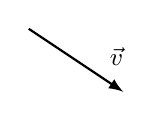
\begin{tikzpicture}[smooth,yscale=-1,xscale=1,scale=.8]
	\tkzInit[xmin=0,xmax=4,ymin=0,ymax=3]
	\tkzClip[space=1]
	\tkzGrid[color=gray!50,step=1]
	\tkzAxeX[above=1pt]
	\tkzAxeY
	\tkzClip[space=.5]

	\draw[-latex,thick] (0,0) -- (1.5,1.0)
		node[near end,above right] {\small $\vec{v}$};
\end{tikzpicture}
\end{center}
\end{multicols}

\vspace*{-4em}
So betrachtet beschreibt uns ein Vektor also nicht nur eine Verschiebung, sondern auch eine Richtung (des Pfeils) und eine Länge (des Pfeils).

Vektoren bieten uns in \programm{Processing} zum Beispiel den Vorteil, dass wir die Koordinaten eines Objektes in nur einer Variablen speichern können. Darüber hinaus lässt sich mit Vektoren aber auch rechnen, was uns viele Aspekte der Grafikprogrammierung erleichtert.

\vspace*{-1em}\subsection*{Vektor zwischen zwei Objekten}
\begin{multicols}{2}
Ist die Position von zwei Objekten $A$ und $B$ durch die Vektoren $\vec{a}$ und $\vec{b}$ beschrieben, dann kann der Vektor von $A$ nach $B$ durch $\vec{b}-\vec{a}$ berechnet werden: \[ \vec{b} - \vec{a} = \vector(b_1|b_2) - \vector(a_1|a_2) = \vector(b_1 - a_1|b_2 - a_2) \]

\begin{center}
\begin{tikzpicture}[smooth,yscale=-1,xscale=1]
	\tkzInit[xmin=0,xmax=4,ymin=0,ymax=3]
	\tkzClip[space=1]
	\tkzGrid[color=gray!50,step=1]
	\tkzAxeX[above=1pt]
	\tkzAxeY
	\tkzClip[space=.5]

	\draw[-latex,thick] (0,0) -- (1.0,2.0)
		node[below left,near end] {\small $\vec{a}$};
	\draw[-latex,thick] (0,0) -- (3.0,1.0)
		node[above,near end] {\small $\vec{b}$};
	\draw[-latex,thick,primary] (1,2) -- (3.0,1.0)
		node[midway,below right] {\small $\vec{b}-\vec{a}$};
\end{tikzpicture}
\end{center}
\end{multicols}

\vspace*{-4em}\subsection*{Vektor zwischen zwei Objekten}
\begin{multicols}{2}
Ein Vektor mit der Länge $1.0$ heißt \emph{normalisiert}. Wenn wir so einen Vektor mit einer Zahl multiplizieren, \emph{skalieren} wir ihn auf eine neue Länge.
\[ \vector(1.0|0.5)\cdot 3.0 = \vector(1.0\cdot 3.0|0.5\cdot 3.0) = \vector(3.0|1.5)  \]

\begin{center}
\begin{tikzpicture}[smooth,yscale=-1,xscale=1]
	\tkzInit[xmin=0,xmax=4,ymin=0,ymax=3]
	\tkzClip[space=1]
	\tkzGrid[color=gray!50,step=1]
	\tkzAxeX[above=1pt]
	\tkzAxeY
	\tkzClip[space=.5]

	\draw[-latex,thick,primary] (0,0) -- (3.0,1.5)
		node[near end,above right] {\small $\vec{v}\cdot 3.0$};

	\draw[-latex,thick] (0,0) -- (1.0,.5)
		node[near end,below left] {\small $\vec{v}$};
\end{tikzpicture}
\end{center}
\end{multicols}

\newpage
\vspace*{-4em}\subsection*{Vektoren in Processing}
\programm{Processing} besitzt eine eigene Klasse, die die Berechnung von Vektoren erlaubt: \code{PVector}\footnote{\url{https://processing.org/reference/PVector.html}}.

\begin{links}[.5]\centering
\begin{minted}{java}
// Vektoren a und b erstellen.
PVector a = new PVector(1.0, 2.0);
PVector b = new PVector(3.0, 1.0);
// Zufälliger Vektor.
PVector c = PVector.random2D();
// Vektor von a nach b berechnen.
PVector ab = PVector.sub(b, a);
// Vektor ab normalisieren (Länge auf 1.0 setzen)
// und dann auf die Länge 3.0 skalieren.
ab.normalize().mult(3.0);
// das geht auch in einem Schritt mit
// setMag (set magnitude).
ab.setMag(3.0);
\end{minted}
% \begin{links}[.66]
% Die vollständige Dokumentaiton der Klasse \code{PVector} findest du in der Processing Referenz.
% \end{links}\hfill\qrlink{https://processing.org/reference/PVector.html}{Referenz der Klasse \code{PVector}.}
\end{links}\begin{rechts}[.5]\centering
	\begin{klassendiagramm}%[show background grid]
		\begin{class}[text width=8cm]{Mover}{0,0}
			\attribute{-position: PVector}
			\attribute{-velocity: PVector}
			\attribute{-acceleration: PVector}
			\attribute{-mass: float}

			\operation{+Mover(pPosition: PVector, pVelocity: PVector, pMass: float)}
			\operation{+update(): void}
			\operation{+draw(): void}
			\operation{+getMass(): float}
			\operation{+getPosition(): PVector}
			\operation{+getVelocity(): PVector}
			\operation{+applyForce(pForce: PVector): void}
		\end{class}
	\end{klassendiagramm}
\end{rechts}

\begin{aufgabe}[subtitle=Gravitation,icon=\iconComputer]
\label{aufg:physik}
\begin{enuma}
	\item
	Erstelle ein neues \programm{Processing} Projekt und speichere es unter dem Namen \ordner{Physik}. Erstelle dann eine Klasse \code{Mover} nach dem Implementierungsdiagramm oben. Nutze die \code{PVector} Klasse für die Position des Movers. Die Darstellung eines Movers mittels der \code{draw} Methode kannst du dir selber überlegen und gegebenenfalls benötigte Attribute ergänzen (z.B. Größe und Farbe).

	Initialisiere die \code{acceleration} (Beschleunigung) zunächst mit einem Nullvektor (\code{new PVector()}).
	\item
	Erstelle im Hauptprogramm die \code{void setup()} und \code{void draw()} Methoden. Erzeuge ein Array mit fünf \code{Mover} Objekten und zeichne sie.
	\item
	{Implementiere die \code{update()} Methode der \code{Mover} so, dass die aktuelle Geschwindigkeit (\code{velocity}) auf die aktuelle Position addiert wird. Aktualisiere die \code{Mover} dann vor dem Zeichnen.

	\hinweis{Implementiere die Aktualisierung in einer eigenen Schleife und nicht in der Schleife zum Zeichnen der \code{Mover}.}}
	\item
	Die Geschwindigkeit eines \code{Mover} wird durch einwirkende Kräfte beeinflusst. Implementiere die Methode \code{applyForce(PVector pForce)} wie folgt:
	\begin{smallitem}
		\item Addiere die Kraft \code{pForce} auf die Beschleunigung (\code{acceleration}).
		\item In der \code{update()}, bevor die Geschwindigkeit zur Position addiert wird:
		\begin{smallitem}
			\item addiere die Beschleunigung auf die Geschwindigkeit (\code{velocity}),
			\item Setze die Beschleunigung auf $(0,0)$.
		\end{smallitem}
	\end{smallitem}
	\item
	Erstelle einen Vektor \code{PVector grav = new PVector(0, 0.06734);} und übergib ihn vor dem Aufruf von \code{Mover.update()} der \code{applyForce()} Methode. Du hast nun eine einfache Simulation der Gravitationskraft implementiert.
	\item
	Initialisiere die \code{Mover} mit einem zufälligen Vektor für die Geschwindigkeit und beobachte, was passiert.
\end{enuma}
\warningbox{Speichere das Projekt an dieser Stelle ab und erstelle eine Kopie mit dem Namen \ordner{Gravitation}, in der du weiter arbeitest. Das Projekt \ordner{Physik} dient als Vorlage für die nächsten Aufgaben.}
\begin{enuma}[resume]
	\item
	Sorge dafür, dass die \code{Mover} am unteren Bildschirmrand abprallen, indem du bei Kontakt eine starke, nach oben gerichtete Kraft anwendest. Du kannst die Stärke der Kraft auch von der Masse des \code{Movers} abhängig machen.

	Um ein Abprallen von den Seiten zu erreichen, reicht es, die Geschwindigkeit in \code{y} Richtung mit \code{-1} zu multiplizieren.
	\item
	Die Stärke der Kraft beim Abprallen am unteren Bildschirmrand und deren Richtung bestimmen, wie das Objekt \enquote{springt}. Ein Gummiball springt stärker als eine Holzkugel. Außerdem spielt die Masse (also das Gewicht) des Objektes eine Rolle. Die Kraft sollte das Objekt außerdem nicht beschleunigen, sondern gerade so stark sein, um seine Richtung zu ändern.

	Implementiere eine Eigenschaft \enquote{Material}, die das \enquote{Sprungverhalten} eines \code{Mover} festlegt.
\end{enuma}
\end{aufgabe}

\newpage
\begin{aufgabe}[subtitle=Kraftstöße,icon=\iconComputer]
\label{aufg:billard}
Die Gravitation ist eine konstante Kraft in eine festgelegte Richtung (nach unten), die auf die \code{Mover} einwirkt. Kräfte können aber aus verschiedenen Richtungen mit variabler Stärke einwirken und die Bewegung der \code{Mover} beeinflussen.

\begin{enuma}
	\item Erstelle eine Kopie deines Physik-Projektes und nenne sie \ordner{Billard}. Entferne im neuen Projekt die Gravitationskraft.
	\item Implementiere eine \code{void mouseClicked()} Methode, die bei einem Mausklick den Movern einen \enquote{Stoß} versetzt.
	\begin{itemize}
		\item Berechne dazu den Vektor von der Mausposition zum \code{Mover}.
		\item Die Länge des Vektors bestimmt die Stärke des Stoßes. Stelle sie auf einen sinnvollen Wert ein (z.B. \code{10.0}).
		\item Benutze den Vektor mit der \code{applyForce} Methode.
	\end{itemize}
	\item Begrenze die Bewegung der \code{Mover} an den Bildschirmrändern, indem du beim Erreichen des Randes die Beschleunigung in die entsprechende Richtung umkehrst.
	\item Eine Billardkugel läuft nach einem Stoß nicht unendlich weit. Die Reibung sorgt dafür, dass sie nach und nach langsamer wird. Setze eine Annäherung dieses Effekts in deiner Simulation um.
	\item Billard funktioniert erst, wenn die Kugeln sich auch gegenseitig beeinflussen können. Implementiere Kollisionen zwischen den \code{Mover} Objekten.

	\begin{links}[.55]
	\begin{itemize}
		\item Prüfe vor dem Aufruf von \code{update()} eines Movers, ob das Objekt mit einer anderen Kugel kollidiert.
		\item Da ein Ball ein Kreis ist, kann eine Kollision einfach ermittelt werden, indem der Abstand zwischen den Mittelpunkten ($m_1$ und $m_2$) der Kugeln berechnet wird. Ist dieser kleiner als die Summe der Radien der Kreise, dann berühren sich diese.
	\end{itemize}
	\end{links}\begin{rechts}[.4]
		\begin{tikzpicture}[scale=.6]
			\begin{scope}[rotate=30]
				% Ball 1
				\draw[fill=primary] (.0,.0) circle (.8);
				\draw[fill=black] (.0,.0) circle (.05);
				% Ball 2
				\def\x{2.4}
				\draw[fill=secondary] (\x,.0) circle (.8);
				\draw[fill=black] (\x,.0) circle (.05);

				% \draw[-,dashed] (0,0) -- (0.4,0.692);
				% \draw[-,dashed] (1.6,0) -- (2,0.692);

				\draw[|-|,dashed] (.0,.0) -- (\x,.0);
				\draw[thick,decorate,decoration = {brace}] (.0,.9) --node[above]{\rotatebox{30}{\tiny$> 2r$}} (\x,.9);
			\end{scope}

			\begin{scope}[shift={(6,.0)},rotate=30]
				% Ball 1
				\draw[fill=primary] (.0,.0) circle (.8);
				\node[below,white] at (.0,.0) {\scriptsize$M_1$};
				\draw[fill=black] (.0,.0) circle (.05);
				% Ball 2
				\draw[fill=secondary] (1.6,.0) circle (.8);
				\node[above,white] at (1.6,.0) {\scriptsize$M_2$};
				\draw[fill=black] (1.6,.0) circle (.05);

				\draw[|-|,dashed] (.0,.0) -- (1.6,.0);
				\draw[thick,decorate,decoration = {brace}] (.0,.9) --node[above]{\rotatebox{30}{\tiny$<= 2r$}} (1.6,.9);
				\draw[-latex,line width=2pt,primary] (.0,.0) -- (-2,.0)
					node[at end,left] {\scriptsize$F_1$};
				\draw[-latex,line width=2pt,secondary] (1.6,.0) -- (3.6,.0)
					node[at end,right] {\scriptsize$F_2$};
			\end{scope}
		\end{tikzpicture}
	\end{rechts}

	\begin{itemize}[resume]
		\item Kollidieren zwei Kugeln, wirkt eine Kraft entgegen der Aufprallrichtung auf beide Kugeln ($F_1$ und $F_2$). Diese entspricht dem Vektor von $M_1$ nach $M_2$ mit einer passenden Länge.
		\item Probiere verschiedene Werte für die Stärke der Kraft aus (also die Länge des Vektors). (Ein sinnvoller Wert ist der Durchschnitt der Aufprallgeschwindigkeiten. Für einen genaueren Wert musst du dich über \emph{Vektorprojektion} informieren.)
	\end{itemize}
	\item
	Mit diesen Grundlagen ist es nun möglich, eine Billardsimulation umzusetzen. Erweitere das Programm nach eigenem Ermessen. Ein Beispiel kannst du dir am Pult zeigen lassen.
\end{enuma}
\end{aufgabe}

\newpage
\begin{aufgabe}[subtitle=Flug der Atome,icon=\iconComputer]
\label{aufg:atome}
\begin{links}[.6]
	Auf unserem Planeten kann die Schwerkraft als eine feste, nach unten gerichtete Kraft definiert werden, die auf die \code{Mover} einwirkt. In unserem relativen Bezugssystem (der Erde) ist dies auch näherungsweise korrekt. Bewegen wir uns allerdings in den Weltraum und betrachten Kräfte zwischen Himmelskörpern, oder ins Atomare und betrachten die Bewegung von Elektronen um einen Atomkern, dann ändern sich die Einflüsse. \person{Isaac Newton} hat diese Kräfte mit seinem Gravitationsgesetz beschreiben.

	\begin{enuma}
		\item Erstelle eine Kopie deines Physik-Projektes aus \prettyref{aufg:physik} und nenne sie \ordner{Atome}. Entferne im neuen Projekt die Gravitationskraft.
		\item Implementiere die Klasse \code{Attractor} nach dem Implementierungsdiagramm rechts. (Für die Methode \code{attract} reicht zunächst ein Gerüst.)
	\end{enuma}
\end{links}\begin{rechts}[.4]\centering
	\begin{klassendiagramm}%[show background grid]
		\begin{class}[text width=6cm]{Attractor}{0,0}
			\attribute{-position: PVector}
			\attribute{-mass: float}

			\operation{+Attractor(pPosition: PVector, pMass: float)}
			\operation{+draw(): void}
			\operation{+getMass(): float}
			\operation{+getPosition(): PVector}
			\operation{+attract(pMover: Mover)}
		\end{class}
	\end{klassendiagramm}
\end{rechts}

\begin{infobox}
	\begin{links}[.6]
	\textbf{Newtonsches Gravitationsgesetz} \\
	Das von \person{Isaac Newton} 1687 definierte Gesetz der klassischen Physik beschreibt die anziehende Gravitationskraft, mit der Massenkörpern aufeinander einwirken. Diese Gravitationskraft ist entlang der Verbindungslinie beider Massenpunkte gerichtet sowie in ihrer Stärke proportional zum Produkt der beiden Massen und umgekehrt proportional zum Quadrat ihres Abstandes.

	\[ F_1 = F_2 = G\cdot \frac{m_1\cdot m_2}{r^2} \]

	Beide Körper ziehen sich also mit derselben Stärke an ($F_1$ bzw. $F_2$). $m_1$ und $m_2$ ist jeweils die Masse der Körper und $G$ die \emph{Gravitationskonstante}.
	\end{links}\begin{rechts}[.4]\centering
	\begin{tikzpicture}[scale=.6]
		\begin{scope}%[rotate=30]
			\def\r{.8}
			\pgfmathsetmacro{\x}{8*\r}
			% Ball 1
			\draw[fill=primary] (.0,.0) circle (2*\r);
			\draw[fill=black] (.0,.0) circle (.05);
			\draw[-latex,line width=2pt,primary] (.0,.0) -- (4*\r,.0);
			\node[primary, above] at (3.2*\r,.0) {$F_1$};
			% Ball 2
			\draw[fill=secondary] (\x,.0) circle (\r);
			\draw[fill=black] (\x,.0) circle (.05);
			\draw[-latex,line width=2pt,secondary] (\x,.0) -- (\x-3*\r,.0);
			\node[secondary,above] at (\x-2.2*\r,.0) {$F_2$};

			\draw[dashed] (.0,.0) -- (.0,-3*\r);
			\draw[dashed] (\x,.0) -- (\x,-3*\r);
			\draw[thick,latex-latex] (.0,-3*\r) --node[above]{$r$} (\x,-3*\r);

			\node[white] at (.0,.0) {$m_1$};
			\node[white] at (\x,.0) {$m_2$};
		\end{scope}
	\end{tikzpicture}
	\end{rechts}
\end{infobox}
\begin{enuma}[start=3]
	\item Implementiere Newtons Gesetz in der \code{attract} Methode so, dass das Objekt \code{pMover} vom \code{Attractor} angezogen wird. (Die umgekehrte Anziehung kannst du ignorieren.)

	Für die Masse der beteiligten Objekte kannst du zunächst \code{50.0} wählen. Die Gravitationskonstante $G$ definierst du als \emph{Klassenvariable} in der Klasse \code{Attractor} mit dem Wert \code{10.0}:
	\begin{minted}[linenos=none]{java}
	public static final float G = 10.0;
	\end{minted}

	\textbf{Hinweise zur Umsetzung:}
	\begin{smallitem}
		\item $r$ bekommst du wieder über die Länge des Differenzvektors. Achte auf die richtige Ausrichtung der Kraft (zum \code{Attractor} hin).
		\item Du musst $r^2$ nicht berechnen. Die Methode \code{magSq} der Klasse \code{PVector} liefert direkt die quadrierte Länge.
		\item Die Anziehung ist vom Abstand $r$ abhängig. Wenn $r = 0$ ist, dann müssten wir durch $0$ teilen, was nicht erlaubt ist. Ist der Abstand sehr klein, dann wird die Kraft unendlich groß. Ist der Abstand wiederum groß, wird die Kraft unendlich klein.

		Um dies zu verhindern, kannst du die \code{constrain} Methode verwenden, um den Abstandswert zwischen einem Minimum und Maximum einzuschränken. Als Richtwerte kannst du zunächst \code{100.0} und \code{1000.0} verwenden.
		\item Damit die Geschwindigkeit nicht viel zu hoch wird, solltest du ihr auch ein Maximum setzen. Dabei hilft dir die \code{limit} Methode der Klasse \code{PVector}.
	\end{smallitem}
	\item Momentan ist die Bewegung der \code{Mover} noch sehr chaotisch. Das liegt daran, dass wir die Masse der Objekte nicht beachten. Ein schweres Objekt sollte langsamer angezogen werden, als ein leichtes. Passe daher die Methode \code{applyForce} so an, dass der Kraftvektor vor Addition zur Beschleunigung durch die Masse geteilt wird.
	\item Erstelle im Projekt einen \code{Attractor}. Rufe \code{attract} einmal mit jedem \code{Mover} vor dessen \code{update} Methode auf.

	Für einen besseren Effekt gib den Movern beim Erstellen eine zufällige Geschwindigkeit. Außerdem könntest du die Farbe und Größe der Objekte abhängig von der Masse oder auch der Geschwindigkeit machen.
	\item Die Gravitationskonstante $G$ bestimmt die Stärke der Anziehung. Verändere sie und auch die Massen der beteiligten Objekte und versuche eine gleichmäßige, gut sichtbare Bewegung der Objekte zu programmieren.

	Ergänze weitere \code{Attractor} Objekte und beobachte, wie sich die Flugbahnen der \code{Mover} verändern. Anstatt zufälliger Positionen und Geschwindigkeit kannst du auch feste Werte nutzen, um interessante Konstellationen zu erstellen.
\end{enuma}
\end{aufgabe}

\newpage
\begin{aufgabe}[subtitle=Vererbungsbeziehungen,icon=\iconComputer]
\label{aufg:vererbung}
\begin{links}[.7]
Bisher beeinflussen sich die Objekte in der Simulation nicht gegenseitig, sondern nur einseitig. Aber was wäre, wenn ein \code{Attractor} auch ein \code{Mover} ist, und von anderen Attractoren angezogen wird?

Diese Art der Beziehung zwischen zwei Klassen (Eine Klasse \code{A} ist auch eine Klasse \code{B}) nennt man \emph{Vererbung}. In unserem Fall ist \code{Attractor} auch ein \code{Mover}. \code{Mover} nennt man die \textbf{Oberklasse} von \code{Attractor}. Umgekehrt ist \code{Attractor} eine \textbf{Unterklasse} von \code{Mover}. (Man spricht auch von einer \emph{Spezialisierung}, da \code{Attractor} ein spezieller \code{Mover} ist.)
\end{links}\begin{rechts}[.3]\centering
	\begin{klassendiagramm}%[show background grid]
		\begin{class}[text width=4cm]{Mover}{0,0}

		\end{class}
		\begin{class}[text width=4cm]{Attractor}{0,-2}
			\inherit{Mover}
		\end{class}
	\end{klassendiagramm}
\end{rechts}

Eine Unterklasse \emph{erbt} alle Attribute und Methoden der Oberklasse. Ein \code{Attractor} braucht also nicht erneut ein Attribut \code{mass} deklarieren, da dies ja schon in \code{Mover} vorhanden ist. Ebenso der passende Getter \code{getMass()}. Die Unterklasse muss nur noch neue Methoden und Attribute implementieren.
\begin{minted}{java}
public class Attractor extends Mover {
	public static final float G = 10.0;

	public Attractor( PVector pPos, float pMass ) {
		// Den Konstruktor der Oberklasse aufrufen
		// "super" bezieht sich immer auf die Oberklasse
		super(pPos, pMass);
	}

	public void attract(Mover pMover) {
		// "self" bezieht sich auf dieses Objekt selbst
		// Differenzvektor bilden
		PVector force = PVector.sub(pMover.getVelocity(), self.getPosition());
		// Länge des Differenzvektors (quadriert) im Intervall
		// [0.01, 100.0] einschränken
		float distSq = constrain(force.magSq(), 100.0, 1000.0);
		// Anziehungskraft berechnen
		float strength = (G * self.getMass() * pMover.getMass()) / distSq;
		// Differenzvektor skalieren und als Kraft anwenden
		pMover.applyForce(force.setMag(strength));
	}
}
\end{minted}
\begin{enuma}
	\item Erstelle ggf. eine Kopie des Projekts aus \prettyref{aufg:atome} oder öffne das Projekt selbst.
	\item Implementiere den \code{Attractor} als Unterklasse des \code{Mover} entlang des Beispiels oben.
\end{enuma}
\begin{links}[.49]
	\begin{enuma}[resume]
		\item Ändere das Hauptprogramm entsprechend des Pseudocodes rechts.
		Für jeden \code{Mover} muss nun \code{attract} von jedem \code{Attractor} einmal aufgerufen werden. Aber Achtung: Da Attractoren nun auch \code{Mover} sind, musst du vor dem Aufruf von \code{attract} prüfen, ob die Objekte gleich sind. In dem Fall passiert nichts, da ein \code{Attractor} sich nicht selber anzieht.
	\end{enuma}
\end{links}\begin{rechts}[.49]
	\begin{minted}[linenos=none]{text}
		ANZAHL_M = 8
		ANZAHL A = 2
		Mover[] movers = new Movers[ANZAHL_M + ANZAHL_A]
		Attractor[] attractors = new Attractor[ANZAHL_A]
		wiederhole mit i von 0 bis ANZAHL_M-1:
			movers[i] = new Mover
		wiederhole mit i von 0 bis ANZAHL_A-1:
			attractors[i] = new Attractor
			movers[ANZAHL_M+i] = attractors[i]
		\end{minted}
\end{rechts}
\begin{enuma}[start=4]
	\item Unterklassen können Methoden ihrer Oberklasse \emph{überschreiben} und so die Funktionsweise ändern. Implementiere in der Klasse \code{Attractor} wieder eine eigene \code{draw} Methode. In der Simulation werden sie nun anders dargestellt, als die \code{Mover}.
	\item Experimentiere mit verschiedenen Werten für die einzelnen Parameter (Massen, Gravitationskonstante, maximale/minimale Kräfte und Geschwindigkeiten, ...).
	\item Entwickele auf der Basis des \code{Attractor} einen \code{Repulsor}, der die Mover von sich abstößt. \\
	Erzeuge zu Beginn nur einige statische Mover. Bei einem Linksklick mit der Maus wird ein \code{Attractor} an der Mausposition erzeugt. Bei einem Rechtsklick ein \code{Repulsor}.
\end{enuma}
\end{aufgabe}

\end{document}
